\documentclass[12pt,twoside]{article}
\usepackage[a4paper,width=150mm,top=30mm,bottom=30mm,bindingoffset=10mm]{geometry}
\linespread{1}
\usepackage[utf8]{inputenc} %Standard diacritics in Romance languages (accents, umlauts)
\usepackage{times} %Uses Times New Roman font
\usepackage{wasysym}
\usepackage{tabularx}
\usepackage{float}
\usepackage{diagbox}
\usepackage{hyperref}
\usepackage{graphicx}
\graphicspath{ {./images/} }
\usepackage[style=authoryear-icomp,natbib=true,sortcites=true]{biblatex}% natbib=true so we can use natbib commands with biblatex
% Also: authoryear-icomp is used so that when you cite the same author with different years, you get "according to Herberger (2002, 2004)" rather than "according to Herberger (2002), Herberger (2004)"
\addbibresource{refs.bib}

\usepackage{xpatch}
\usepackage{listings}
\usepackage{color}

\definecolor{dkgreen}{rgb}{0,0.6,0}
\definecolor{gray}{rgb}{0.5,0.5,0.5}
\definecolor{mauve}{rgb}{0.58,0,0.82}

\lstdefinestyle{scala}{frame=tb,
language=Scala,
aboveskip=3mm,
belowskip=3mm,
showstringspaces=false,
columns=flexible,
basicstyle={\small\ttfamily},
numbers=none,
numberstyle=\tiny\color{gray},
keywordstyle=\color{blue},
commentstyle=\color{dkgreen},
stringstyle=\color{mauve},
breaklines=true,
breakatwhitespace=true,
tabsize=3}

\lstdefinestyle{cpp}{frame=tb,
language=C++,
aboveskip=3mm,
belowskip=3mm,
showstringspaces=false,
columns=flexible,
basicstyle={\small\ttfamily},
numbers=none,
numberstyle=\tiny\color{gray},
keywordstyle=\color{blue},
commentstyle=\color{dkgreen},
stringstyle=\color{mauve},
breaklines=true,
breakatwhitespace=true,
tabsize=3}

\lstset{style=scala}


\usepackage[tiny]{titlesec}
\titleformat{\subsection}{}{\thesubsection}{1em}{\itshape}
\titleformat{\subsubsection}{}{\thesubsubsection}{1em}{\itshape}
\titlelabel{\thetitle.\quad}

\usepackage{fancyhdr}
\pagestyle{fancy}
\fancyhead{}
\fancyhead[LE]{\thepage \hspace{3mm} \small }
\fancyhead[RE]{\small Nassouh AlOlabi}
\fancyhead[LO]{\small Complex State Management with Immutability}
\fancyhead[RO]{\small  \normalsize \thepage}
\fancyfoot{}
\setcounter{page}{-3} %This sets the initial page at a number other than 1 (in this case 23).

\fancypagestyle{first}{
	\fancyhead{}
	\fancyhead[L]{\small Higher Institute for Applied Sciences and Technology \\\url{https://hiast.edu.sy}\\{}}
	\fancyhead[R]{\small IT Dept. 2022, \\{}}
	\fancyfoot{}}
	%don't worry about the headers, we will compile them

\fancypagestyle{cluster}{
    \fancyfoot[L]{\rule[10pt]{430pt}{1pt} \\{} \small (1) Cluster: is a set of computers that work together so that they can be viewed as a single system.\\{} which allows us to scale horizontally with commodity hardware effectively.\\{} \small (2) DOM: Document Object Model.}
    }
    

\newcommand{\pref}[1]{(\ref{#1})} % If you use \ref{xx}, the reference in the text appears without parentheses: "as we see in 1, ..." instead of "as we see in (1)...". So we create a new command: instead of \ref, call \pref (Parentheses REFerence) which specifies that any cross references to xx appear in parentheses.

\usepackage{tipa} %for IPA
\usepackage{phonrule} %for phonological rules
\usepackage[nocenter]{qtree} %for trees
\usepackage{gb4e} %for examples and glossing

\usepackage[normalem]{ulem} %STRIKETHROUGH TEXT

\usepackage{authblk,etoolbox}
\renewcommand\Authfont{\Large}
\renewcommand\Affilfont{\normalsize}

\makeatletter
% patch \maketitle so that it doesn't center
\patchcmd{\@maketitle}{center}{flushleft}{}{}
\patchcmd{\@maketitle}{center}{flushleft}{}{}
% patch \maketitle so that the font size for the title is normal
\patchcmd{\@maketitle}{\LARGE}{\normalsize}{}{}

\def\maketitle{{%
		\renewenvironment{tabular}[2][]
		{\begin{flushleft}}
			{\end{flushleft}}
		\AB@maketitle}}
\makeatother

\title{\Huge{Complex State Management with Immutability}}
\author{Nassouh AlOlabi} 
\affil{Scientific supervisor: Dr.Yasser Rahal}
\affil{General supervisor: Dr.Kadan Joumaa} 
\affil{Linguistic supervisor: Fahmi Alammareen}
\setlength{\affilsep}{1pt}
\date{}

%IF THERE ARE TWO AUTHORS:
%\title{\Huge{Patterns of syntactic microvariation: the case of European Portuguese}}
%\author{Noam Chomsky} \affil{Massachusetts Institute of Technology\\noam.chomsky@mit.edu} 
%\author{Howard Lasnik} \affil{University of Maryland\\howard.lasnik@umd.edu}
%\setlength{\affilsep}{1pt}
%\date{}

\begin{document}

\pagenumbering{Roman}

\begin{figure}
    {
\includegraphics[scale=.25]{logo.png}}
\end{figure}

\maketitle

\thispagestyle{first}

\vspace{0.5cm}

\hfill Received: 22-02-2022 

\hfill Accepted: 25-02-2022

\hfill Published: 05-03-2022

\vspace{1cm}

% \noindent \textbf{How to cite} Leave blank

\vspace{1.5cm}
\newpage
\noindent \textbf{Abstract}
\newline\newline
% \begin{center}
%  	\line(1,0){430}
% \end{center}
% \vspace{-0,3cm}
\noindent Growing demand for fault-tolerant, scalable, distributed systems has made some mainstream software architectures and patterns obsolete or rather harder to come by, Thus came the rise of stateless and functional solutions based on data immutability which has already been the cornerstone of Big Data [1]. We'll take a deep look at immutability and how it should look like in a system, then we will view four emerging technologies that implement immutability in some form and how it made them standout in the industry.

\vspace{5mm}

\noindent \textbf{Keywords:} immutable data structures, functional programming, algorithm design

\vspace{4mm}
% \begin{center}
% 	\line(1,0){430}
% \end{center}

% \begin{center}
% 	\textbf{Table of Contents}
% \end{center}

% \begin{large}
% \begin{center}
% 	\begin{tabular}{c c}
% 		1. Section 1 & 4. Section 4\\
% 		2. Section 2 & 5. Section 5\\
% 		3. Section 3 & 6. Section 6
% 	\end{tabular}
% \end{center}
% \end{large}

\newpage
\tableofcontents
\newpage

\pagenumbering{arabic}
\setcounter{page}{1}

\newpage
\section{Introduction}
% immutability an empircal study in scala
Unintended mutations of a program’s state cause inconsistent behavior and bugs of the
program. These mutations might have been introduced by side-effects of functions that developers
were unaware of during the program’s implementation. Some programming languages do, for example,
allow arguments of a function to be mutated. The fact that a third-party function can mutate the
state of its argument can go undetected. The problem of rogue and complicated state mutations can
become difficult to handle when states are shared among objects. One way to avoid undesired mutations
is to use immutable data instead of mutable data. Immutable data cannot be mutated once created
and instead of mutating shared data in memory, data would have to be re-created to include the modifications
needed. Programmers can then safely share data without the possibility of having it mutate to
something else, which is crucial to avoid, for example, race conditions in concurrent programs.

\newpage
\section{State Management}
% https://medium.com/super-declarative/understanding-state-management-and-why-you-never-will-dd84b624d0e
The term state management has gain traction over the last decade or so with the emergence of wide spread IT solutions and the ease of making one of your own from whatever background you come from. Depending on the underlying scenario the term could stand for:
Data persistence management,
Information flow,
Programming paradigms,
I/O (especially networking and caching), %% TODO: latency table
Application architecture,
Presentation behavior and 
UI templating. Therefore the term state management has been a catch-all term from data modeling to parallel computing. 

\subsection{Data Persistence}

%%-----------https://www.researchgate.net/publication/221596019_Analyzing_persistent_state_interactions_to_improve_state_management ---------
A primary challenge to building reliable and secure computer systems is managing the persistent state of the system: all the executable files, configuration settings and other data that govern how a system functions. The difficulty comes from the sheer volume of this persistent state, the frequency of it's changes, and the variety of workloads and requirements that require customization of persistent state. The cost of not managing a system's persistent state effectively is high: configuration errors are the leading cause of downtime at Internet services, troubleshooting configuration problems is a leading component of total cost of ownership in corporate environments, and malware—effectively, unwanted persistent state—is a serious privacy and security concern on personal computers.
%In this paper, we analyze how computer systems dynamically interact with files and configuration settings in an attempt to gain insights into the problem of persistent state management. We analyze over 3648 machine days of these persistent state interactions, collected over an 8 month period from 193 machines. These machines are under real workloads and include Internet servers, corporate desktops, and home machines. We characterize the scope and magnitude of the persistent state management problem today, measuring not only the gross characteristics of persistent state, but also analyzing how it is used by applications, and when administrators and users modify it. We find that monitoring persistent state interactions provides important visibility and show how it can be used as a foundation for building better persistent state management tools.
%%----------------------------------------------------

\subsection{Information Flow}
%%https://thedaylightstudio.com/blog/2018/03/14/what-is-state-in-web-application-development
Application State (a.k.a. Program State) represents everything necessary to keep your application running.  When we refer to application state we are normally referring to the state of the program as exists in the contents of its memory.  What does that mean practically?  How am I to understand that?  It helps to think in extremes.  What happens to information and functionality core of your application if a server goes down and restarts?  You lose whatever was residing in memory.

%This is one of the reasons why in web development we often use stateless resource controllers which disseminate the information necessary to the running of your application in a way that does not rely heavily on holding data for retrieval on the server’s memory.
%% -------------------------------

%% https://dojotoolkit.org/documentation/tutorials/1.6/data_modeling/
 %The Model-Viewer-Controller (MVC) is a dominant paradigm for application development. The MVC approach separates key common concerns for organized, manageable application code. Dojo is heavily based on MVC principles, and provides powerful helpers for MVC-structured applications. The foundation of a well-designed MVC application is a solid data model. Here we will see how we can leverage Dojo object stores and Stateful objects to create a robust model that can be used in the view and controller code. The model is the M in MVC. The data model represents the core information that your application is being used to access and manipulate. The model is the center of your application
%%--------------------------------------



%%%%https://www.researchgate.net/publication/2716493_The_Role_of_Distributed_State
%Distributed state offers the potential for improving the performance, coherency, and reliability of distributed systems. Unfortunately, distributed state also introduces consistency problems, crash sensitivity, time and space overheads, and complexity; these problems make it difficult to achieve the potential benefits. This paper describes the advantages and disadvantages of distributed state, and presents the NFS and Sprite file systems as examples of different tradeoffs. It does not appear possible to achieve all the advantages of distributed state and also avoid all the problems; rather, system designers must make compromises based on the needs of their individual environments. The Role of Distributed State February 19, 1990 1. Introduction Webster's New World Dictionary defines state as "a set of circumstances or attributes characterizing a person or thing at a given time" [4]. State plays a fundamental role in all computer systems. One way of characterizing computation is as a ...
%----------------

Anti-Patterns or pitfalls includes[2]:

% http://www.padsweb.rwth-aachen.de/wvdaalst/publications/p514.pdf
\subsubsection{Missing Data}
It is the situation where some data element needs to be accessed, i.e. read or destroyed, but either it has never been created or it has been deleted without having been created again.
\subsubsection{Inconsistent Data} 
Data is inconsistent if a task is using this data while some other task (or another instance of the same task) is writing to this data or is destroying it in parallel.
%-----------------------------
\subsection{Programming Paradigms}
% https://www.geeksforgeeks.org/introduction-of-programming-paradigms/
Programming paradigm is an approach to solve problems using some programming languages. It is also a method to solve a problem using available tools and techniques.
%----------------------------------------
Most paradigms have their own opinion on data manipulation for example: Procedural \& Object Oriented paradigms allow more access to data modifying (destructive updates), deleting. Others like Logic \& Functional does not allow these modifications and deletions.

\subsection{I/O, Network and Disk}
% https://www.solarwinds.com/-/media/solarwinds/swdcv2/licensed-products/storage-resource-monitor/resources/whitepapers/top_4_causes_of_storage_io_bottlenecks.ashx
Applications that are I/O heavy often cause bottlenecks. I/O intensive applications are more sensitive to a storage latency issue. When you have a large user base trying to access these applications, slowdowns tend to take place. Increased response time in storage I/O causes bottlenecks. When there is a queue in the storage I/O, you would generally see an increase in latency.
% TODO: often times
Network and Disk latency are often times the biggest source of headache if poorly managed, which is often times the case since they're usually treated as if they were function calls which they're clearly not [3].
% http://norvig.com/21-days.html#answers
\begin{center}
    \begin{table}[H]
        \begin{center}
        \begin{tabularx} {0.8\textwidth}{ 
            | >{\raggedright\arraybackslash}X 
        | >{\raggedleft\arraybackslash}X | }
        \hline
        execute typical instruction &	1/1,000,000,000 sec = 1 nanosec\\
\hline
    fetch from L1 cache memory &	0.5 nanosec\\
\hline
branch misprediction &	5 nanosec\\
\hline
    fetch from L2 cache memory &	7 nanosec\\
\hline
    Mutex lock/unlock &	25 nanosec\\
\hline
    fetch from main memory &	100 nanosec\\
\hline
    send 2K bytes over 1Gbps network &	20,000 nanosec\\
    \hline
    read 1MB sequentially from memory &	250,000 nanosec\\
\hline
    fetch from new disk location (seek) &	8,000,000 nanosec\\
\hline
    read 1MB sequentially from disk &	20,000,000 nanosec\\
\hline
    send packet US to Europe and back &	150 milliseconds = 150,000,000 nanosec\\
    \hline      
    % \float
\end{tabularx}
    
\end{center}
\caption{ \label{tab:1} Latency numbers every programmer should know[4]}
\end{table}
\end{center}
As you can see disk fetches can take 100x more than main memory fetches. When dealing with distributed systems where network call are integral parts of the system, treating network calls which are 100000x more than main memory calls ends up with catastrophically unpredictable behavior



%-------------------------------------------------------


%this format problems tech solutions
\newpage
\section{Immutability}


% src
% Immutability an Empirical Study in Scala.pdf
When something is immutable, we say that it cannot be changed or that it is unchangeable. An immutable object in an object-oriented programming language is an object that has a state that cannot be mutated once instantiated (created). Moreover, an immutable class is a class whose instances cannot be mutated, meaning that there are no methods in the class that can mutate an instance of it. Classes that are not immutable can have instances that are immutable. 

\subsection{Forms of Immutability}
There are different varieties of immutability used today. They includes:
\begin{itemize}
    \item Object immutability
    \begin{description}
        \item[] An immutable object is an object that cannot be modified (mutated), i.e., its state cannot be mutated
    \end{description}
    \item Class immutability 
    \begin{description}
        \item[] When every instantiated object of a class is immutable, then we say that the class itself is immutable.
    \end{description}
    \item Deep and shallow immutability (transitivity)\begin{description}
        \item[] Immutability can be deep or shallow, i.e., transitive or non-transitive:
        \item[]Deep (transitive): immutability means that all objects referred to by an immutable object must also be immutable.
        \item[]Shallow (non-transitive) immutability has a more relaxed constraint, and the immutable object may refer to objects that are mutable, but the fields of the immutable object itself cannot be mutated.
    \end{description}    
    \item Reference immutability (read-only references)
     \begin{itemize}
    \item[] Languages with the support of reference immutability have the notion of read-only references. A readonly reference cannot mutate the object it refers to. When all references to an object are readonly, then nothing can mutate the object, and the object is immutable. There is no guarantee that a referred to object is immutable because the object may still be mutated by some other references that are not read-only, unless there is some analysis that ensures that there only exist readonly references to that object. Reference immutability thus often ensures shallow (non-transitive) immutability and “reference immutability” does not mean that a reference itself is immutable [5].
\end{itemize}


\item Non-assignability
     \begin{itemize}
    \item[] Non-assignability is a form of immutability and property of a variable that makes sure that the variable cannot be reassigned. Since fields of objects are variables and if no variable can be reassigned after its initial assignment, the object is effectively immutable if what the fields are referring to is immutable. This makes non-assignability give shallow (non-transitive) immutability too. Assignment of an object’s field mutates the object, but it does not mutate what was previously on the field or what was assigned to the field.
\end{itemize}


\item Concrete and abstract immutability
     \begin{itemize}
    \item[] Concrete immutability does not allow any change to the object’s state. Abstract immutability, however, allows an immutable object to change its internal state but not the object’s “abstract” value. The object is still immutable from the perspective of the object’s observer, who can only see the abstract value, but the object may mutate internally. This can, for example, be useful to speed up certain operations, lazy initialization and buffering.
\end{itemize}


\end{itemize}

\subsection{Properties of Immutability}
% write some problems
% The concept of immutability is important and
Utilizing immutable data is considered to ease software development and reasoning about programs in
numerous ways, for example:

\subsubsection{Predictability} It is hard to understand and reason about programs that have shared mutable
states with unclear interactions. Tracking mutations and maintaining the correct state of a program
can be difficult. Using immutable data naturally, avoids state changes and forces the programmer
to let data flow and be utilized in a different way throughout the program, making the state of the
program more predictable. For example, calling the same function twice would yield the same result,
and the outcome is predictable. Without the immutability guarantee, the second call could
yield another result because of an underlying state mutation making it less predictable.

\subsubsection{Testability} Because immutable data can only be changed once during construction, they are inherently
simpler and easier to unit test. One may reason that by restricting the number of possible mutations
in a program; the number of potential errors of the program is also reduced. Testing is essentially
to validate that mutations in the program occur correctly and thus having more mutations would require more testing. By restricting the number of mutations in a program, the program has
fewer causes of errors to occur and there will be fewer state transitions to test.

\subsubsection{Concurrency} Immutable data are thread-safe. As data cannot mutate, there is no danger in having
multiple threads access the same data at the same time and have synchronization issues.

\subsubsection{Modularity} Without depending on a local or global state, immutable types and data may be reused
in different contexts more easily.

\newpage
\section{Methods}

\subsection{Reassignment}
There's a subtle difference, well
hidden behind the overloaded use of the symbol
‘=’, that really sets the two apart. In the imperative
program, ‘=’ refers to a destructive update; assigning
a new value to the left-hand-side variable,
whereas in the functional program ‘=’ means true
equality, and that both the left-hand-side and the right-hand-side can be used interchangeably. This characteristic
of functional programming (known as referential
transparency or purity) has a profound influence
on the way programs are constructed and reasoned
about.

% TODO: My definition:
% before we move on it's important to do the distinction between mutation and Reassignment. simply put when you mutate data the old version of it would become unusable and simple would cease to exist. On the other hand updating a variable should keep the old version usable. a perfect example of this is a VCS (version control system) it gives you the feeling that you are mutating files while in fact it's storing changes (updates) and updating a "HEAD" value to represent the last change (update)


\subsection{Shadowing}

Shadowing is a technique that could be used to represent a changing variable, like an accumulator. This technique is simple and possible in almost every programming language.
At its simplest form, shadowing looks like this:
\begin{lstlisting}
    scala> object Main {
        def main(args: Array[String]) = {
            val i = 1;
            {
                val i = 2;
                {
                    val i = 3;
                }
            }
        }  
    }    
\end{lstlisting}
But that's not really useful and even more confusing and very error prone. You are right. shadowing in itself isn't really useful. but it is really at the core of any recursive solution since every function come with its own block and 
\begin{lstlisting} 
    scala> def factorial (n: BigDecimal):BigDecimal = {
        if (n <= 1)  1
        else n * factorial(n-1)
    }
\end{lstlisting}
Notice here n value ranges over \{n, ... , 1\} but it isn't really changing... each n deffer from the other and has it's own scope
if you run this code it'll only go so far (around  n = 9613 for this example) until you get a StackOverflowError... not good.




\subsection{Tail Recursion}
Tail recursion provides stack safety to our solutions and prevents Stackoverflows. It is when you simply return the value of a function call at the end (tail) of your function. in other words, your function has done its job and hands over the rest of the work to another function.
\begin{lstlisting}
  def factorial (n: BigDecimal):BigDecimal = {
    def helper(n: BigDecimal, Acc: BigDecimal): BigDecimal = {
      if (n <= 1) Acc
      else helper(n - 1, n * Acc)
    }
    helper(n, 1)
  }
\end{lstlisting}
Notice that as n takes the values \{n, n-1, n-2, ...\}
the accumulator also changes \{n, n*(n-1), n*(n-1)*(n-2), ...\}
which is very similar to a for loop accumulator pattern, so similar that sometimes compilers compile tail recursive functions to an actual loop


\subsection{Pure Functions}
Pure Functions serve as a (possibly infinite) lookup table mapping from one type to another since variable $x$ will always be the same, $f(x)$ will be the same too. this is what's known as referential transparency.
\lstset{style=cpp}
\begin{lstlisting}
    #include <functional>
    #include <iostream>
    int sum(const int v[], const int& n) {
        std::function<int(int, int)> helper = [&v, &n, &helper](int index, int Acc) {
            if (index >= n) return Acc;
            return helper(index + 1, Acc + v[index]);
        };
        return helper(0, 0);
    }
    int main(int, char**) {
        const int a[] = {1, 2, 3, 4, 5, 6};
        // a[1] = 3; not allowed
        int total = sum(a, 6); // 21
        someFunction(a);
        otherFunction(a);
        if (total == sum(a,6))
            std::cout<<"It should be equal same function same argument?!";
        return 0;
    }
\end{lstlisting}
generally speaking $"someFunction"$ and $"otherFunction"$ could've done all sorts of things with $a$ (changing an element value, adding more elements, removing some elements, delete the pointer entirely ...). If they were pure functions or like in this case using some sort of a language guarantee (here it's $const$) $a$ will not be modified and in turn $total == sum(a,6)$ and overall, our program would be easier to reason about.

\subsection{Laziness}
sometimes referred to as call-by-need, it's the notion that "if data won't change neither will function outputs " meaning that we wouldn't perform any operation unless it is absolutely necessary 
\lstset{style=scala}
\begin{lstlisting}
    def from(n: Int): LazyList[Int] = 
        n #:: from(n+1) 
        // here from(n+1) won't be evaluated
    def sieve (s: LazyList[Int]): LazyList[Int] = 
        s.head #:: sieve(s.tail.filter(_ % s.head != 0)) 
    // nor would sieve(s.tail.filter(_ % s.head != 0))
    val primes = sieve(from(2))

    primes
        .take(10)
        .toList // now it's necessary

\end{lstlisting}
In this example only 10 elements of the infinite "LazyList" are evaluated. The other elements are immutable they are yet to be evaluated and materialized.
% \subsection{Copy-On-Write (COW)}
% https://en.wikipedia.org/wiki/Copy-on-write
% https://www.researchgate.net/publication/220143982_Effects_of_Copy-on-Write_Memory_Management_on_the_Response_Time_of_UNIX_Fork_Operations

\subsection{Structural Sharing}
While imperative programmers are very careful with passing references around and often times rely on cloning. on the other hand persistent data structures allows for more flexibility and safety in sharing and reusing data with ease.
\begin{figure}[H]
    \begin{center}
        {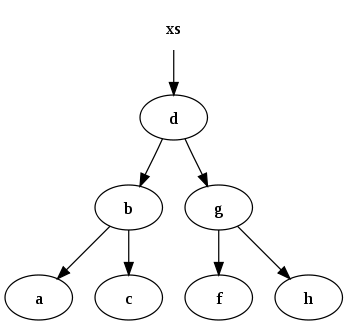
\includegraphics[scale=.65]{originalTree.png}}
    \end{center}
    \caption{ \label{figure:1} Original BST for the corresponding values [a,b,c,d,f,g,h]}
\end{figure}
now what if you wanted to add Node(e) to our Binary Search Tree. now if we were to naively implement an algorithm that would insert the node without mutation is to clone the tree and afterwards do the desired mutations. on the other hand if we consider immutability as and advantage we'll take into account that unaffected node (nodes that we don't need to modify e.g. nodes b,a,c,h) would never change and we can safely reuse them.
\begin{figure}[H]
    \begin{center}
        {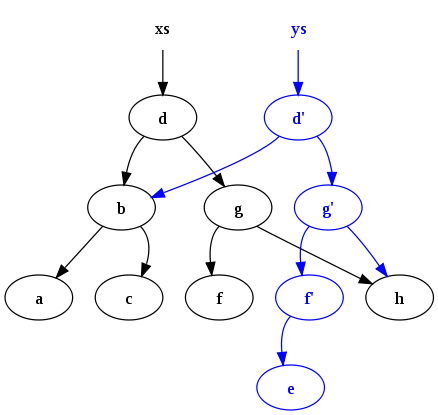
\includegraphics[scale=.6]{structuralSharing.png}}
       \end{center}
       \caption{ \label{figure:2} Resulting BST ys which shares most of the elements in xs}
\end{figure}
Structural Sharing is a very powerful technique and is the core concept for many of optimization techniques such as Copy-on-write paging strategies for address space
inheritance have been shown to be effective in reducing the
real time required to perform UNIX fork() operations. This reduction in copying also reduces the amount of
swap space required, reduces the amount of time spent swapping, increases the number of processes which can be run
without paging, and decreases the cost of context switches.[6]


\newpage
\section{Solutions}
% me<<<
% Incorporating Immutability as a key architectural concept throughout memory layers in a system is

% immutability changes everything<<<
% The trend to leverage immutability in new designs is so pervasive we see it in a number of hardware areas. We first examine the implementation of SSDs, then some new trends in hard disks

% mix<<<
The trend to leverage immutability as a key architectural concept in new designs is so pervasive we see it in a number of new technologies and open source projects, we'll go through the same four areas of state management and see flagship technologies that leverage immutability in some of their features:

\subsection{Copy-on-Write File Systems}
% COW based file Systems pdf
COW generally follows a simple principle. As long as multiple programs need read only access to a data structure, providing them only pointers[7] which point to the same data structure, instead of copying the whole structure to a new one, is enough. If at least one of the programs needs at some point write access to the data structure, create a private copy for it. The same holds for each one of the programs which will need write access to the data structure. A new private copy will be created for them. Note that the unchanged data can still be shared between both programs. COW file systems also provides many other powerful features, But our main interest for this paper is only one of them which is snapshots.
% Most COW-based file systems provides the ability to take snapshots of your files.

A snapshot is a consistent image of the data at a specific point in time. By data I mean the contents of a Fle system, the contents of a database, etc. Snapshots can be read only, or read/write. Writable snapshots are also called clones. Snapshots are extremely useful and have many applications: data recovery, online data protection, undo Fle system operations, testing new installations and configurations, backup solutions, data mining, and more. 

% Leveraging immutability in the implementation snapshots
% https://repositum.tuwien.at/handle/20.500.12708/10774
One of the uses of the snapshot is for enabling of consistent backups. A backup can get inconsistent if during the backup the file system is used. Another use of the snapshot is that the snapshot is kind of easy backup that allows for the retrieving of removed or changed data. Taking of snapshots can be set up in this way that file system could do multiple level undoes. Especially if taking of snapshots does not affect performance of the system[8].

% https://docs.oracle.com/cd/E19253-01/819-5461/gbcxc/index.html
When a snapshot is created, its disk space is initially shared between the snapshot and the file system, and possibly with previous snapshots. As the file system changes, disk space that was previously shared becomes unique to the snapshot, and thus is counted in the snapshot's used property. Additionally, deleting snapshots can increase the amount of disk space unique to (and thus used by) other snapshots.

A snapshot's space referenced property value is the same as the file system's was when the snapshot was created.

You can identify additional information about how the values of the used property are consumed. New read-only file system properties describe disk space usage for clones, file systems, and volumes.

% https://www.youtube.com/watch?v=lsFDp-W1Ks0 --not immutablility realated
% last dacade disk size grow almost 8 folds --not immutablility realated
% while speed almost doubled --not immutablility realated

\subsection{Kafka}
Apache Kafka® is an event streaming platform. And in order to understand what it does and how it leverages immutability in it's architecture we first have to understand what event streaming is. In short, it's the practice of capturing data in real-time from event sources like databases, sensors, mobile devices, cloud services, and software applications in the form of streams of events; storing these event streams durably for later retrieval; manipulating, processing, and reacting to the event streams in real-time as well as retrospectively; and routing the event streams to different destination technologies as needed. Event streaming thus ensures a continuous flow and interpretation of data so that the right information is at the right place, at the right time.[10]


Kafka relies on a publish/subscribe messaging system. It is often described as a “distributed commit log” or more recently as a “distributing streaming platform.” A filesystem or database commit log is designed to provide a durable record of all transactions so that they can be replayed to consistently build the state of a system. Similarly, data within Kafka is stored durably, in order, and can be read deterministically. In addition, the data can be distributed within the system to provide additional protections against failures, as well as significant opportunities for scaling performance.[9]

% https://developer.confluent.io/learn-kafka/apache-kafka/partitions/#:~:text=Kafka%20Partitioning&text=Partitioning%20takes%20the%20single%20topic,many%20nodes%20in%20the%20cluster.
Part of what makes Kafka scale so well is that It gives us the ability to partition topics. Partitioning takes the single topic log and breaks it into multiple logs, each of which can live on a separate node in the Kafka cluster\textsuperscript{1}. This way, the work of storing messages, writing new messages, and processing existing messages can be split among many nodes in the cluster.

\thispagestyle{cluster}


% https://stackoverflow.com/questions/58224758/what-does-it-really-mean-by-kafka-partitions-are-immutable#:~:text=Tha%20Kafka%20partitions%20are%20defined,a%20producer%20point%20of%20view.
Tha Kafka partitions are defined as "immutable" referring to the fact that a producer can just append messages to a partition itself and not changing the value for an existing one (i.e. with the same key). The partition itself is a commit log working just in append mode from a producer point of view. Of course, it means that without any kind of mechanisms like deletion (by retention time) and compaction, the partition size could grow endlessly. At this point you could think .. "so it's not immutable!" as you mentioned. Well, as I said the immutability is from a producer's point of view. Deletion and compaction are administrative operations. For example, deleting records is also possible using the Admin Client API ... but we are always talking about administrative stuff, not producer/consumer related stuff.
If you think about compaction and how it works, the producer initially sends, for example, a message with key = A and payload = "Hello". After a while in order to "update" the value, it sends a new message with same key = A and payload = "Hi" ... but actually it's a really new message appended at the end of the partition log; it will be the compaction thread in the broker doing the work of deleting the old message with "Hello" payload leaving just the new one. In the same way a producer can send the message with key = A and payload = null. It's the way for actually deleting the message (null is called "tombstone"). Anyway the producer is still appending a new message to the partition; it's always the compaction thread which will delete the last message with key = A when it saw the tombstone.


\subsection{Elm}

A delightful language
for reliable web applications[11].
Elm uses The Model-Viewer-Controller (MVC) which is a dominant paradigm for application development. However Elm has an added bonus of Models being immutable. 
\subsubsection{Introduction}
% https://www.sitepoint.com/functional-reactive-programming-elm-introduction/
% \subsubsection{Describe State Instead of Transforming the DOM}
% Not long ago we were building applications by mutating the DOM manually (e.g. using jQuery). As our application grows we introduce more states. Having to code the transformations between all of them exponentially grows the complexity of our application making it harder to maintain.


In web development it's quite common to describe state changes by mutating the DOM\textsuperscript{2} manually. And because of that as the application  grows the transformations we write would grow exponentially with it, making the code harder and harder to maintain. Instead of that, modern libraries have popularized the notion of focusing on describing a particular DOM state and then let the library handle the DOM transformations for us. We only focus on describing the discreet DOM states and not how we get there. This leads to substantially less code to write and maintain.

% \subsubsection{Events and Data Transformation}
When it comes to application state, the common thing to do was to mutate the state ourselves e.g. adding comments to an array.
Instead of doing this we can only describe how the application state needs to change based on events, and let something else apply those transformations for us.

The benefit of doing this is that we can write ‘pure’ functions to describe these transformations. These functions are easier to understand and test. An added benefit is that we can control where our application state is changed, thus making our applications more maintainable. Another benefit is that our views don’t need to know how to mutate state, they only need to know what events to dispatch.

% \subsubsection{Unidirectional Data Flow}
% Another interesting trend is having all our application events flow in a unidirectional way. Instead of allowing any component talk to any other component, we send message through a central message pipeline. This centralized pipeline applies the transformations we want and broadcasts the changes to all the parts of our application. Flux is an example of this.

% By doing this we gain more visibility of all interactions that happen in our application.

% \subsubsection{Immutable Data}
Mutable data makes it very hard to restrict where it can be changed, as any component with access to it could add or remove something. This leads to unpredictability, as state could change anywhere.

By using immutable data we can avoid this, by tightly controlling where application state is changed. Combining immutable data with functions that describe the transformations gives us a very robust workflow, and immutable data helps us enforce the unidirectional flow by not letting us change state in unexpected places.
% \subsubsection{Centralized State}

It's a known fact that Centralized State specifically Global variables are an indication of hard to maintain code. However Having an Immutable Central State is quite different. The use of a centralized ‘atom’ for keeping all state. Meaning that we put all state in one big tree instead of having it scattered across components has become a trend in web development.
In a typical application we usually have global application state (e.g. a collection of users) and component specific state (e.g. the visibility state of a particular component). It is controversial whether storing both kinds of state in one place is beneficial or not. But at least keeping all application state in one place has a big benefit, which is providing a consistent state across all components in our application.
\subsubsection{Where Elm Shines}
elm-html -the part of Elm which render(produce) the corresponding html code to what you write in Elm- are based on the virtual-dom project, which is responsible for the great performance. 
This library is based on the idea of a “virtual DOM”. Rather than touching the DOM directly, we build an abstract version of it on each frame. We use the node function to create a cheap representation of what we want. Virtual DOM sounds pretty slow, right? Create a whole new scene on every frame? This technique is actually widely used in the game industry and performs shockingly well for DOM updates when you use two relatively simple techniques: diffing and laziness.

Diffing to figure out how the DOM needs to be modified. Diffing means taking the current virtual DOM and the new virtual DOM and looking for changes. It sounds kind of fancy at first, but it is a very simple process. We first make a big list of all the differences, like if someone has changed the color of a particular part of the screen or added an entirely new one. After all of the differences are found, we use them as instructions for modifying the DOM in one big batch. This means we do the dirty work of modifying the DOM and making sure everything is fast. You can focus on writing code that is easy to understand and maintain.
This approach created a clear path to fully supporting HTML in a way that is perfect for Elm! Even better, Elm already has great facilities for purity and immutability, which are vital for optimizations that make diffing way faster.
Being lazy about diffing can lead to great performance improvements, especially if you have immutable data. For example, let’s say we are rendering a list of tasks:

But we may know that on many updates, none of the tasks are changing. And if no task changes, the view must not be changing either. This is a perfect time to be lazy:
Instead of calling the todoList function on every frame, we check to see if state.tasks has changed since last frame. If not, we can skip everything. No need to call the function, do any diffing, or touch the DOM at all! This optimization is safe in Elm because functions are pure and data is immutable.
Purity means that the todoList function will always have the same output given the same input. So if we know state.tasks is the same, we can skip todoList entirely.
Immutability makes it cheap to figure out when things are “the same”. Immutability guarantees that if two things are referentially equal, they must be structurally equal.
So we just check to see if todoList and state.tasks are the same as last frame by comparing the old and new values by reference. This is super cheap, and if they are the same, the lazy function can often avoid a ton of work. This is a pretty simple trick that can speed things up significantly.
\begin{figure}[H]
    \begin{center}
        {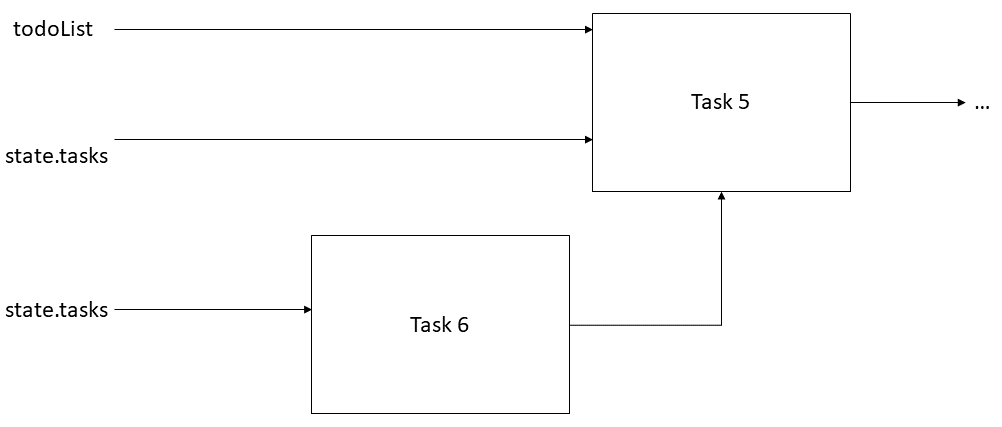
\includegraphics[scale=0.55]{refeq.png}}
       \end{center}
       \caption{ \label{figure:3} A new Task was added to state.tasks and according to what we learn from a previous section about structural sharing we know the before and after the add operations our lists would look like this.}
\end{figure}
If you have been following Elm, you may begin to see a pattern: purity and immutability are kind of a big deal.

Performance is a good hook, but the real benefit is that this approach leads to code that is easier to understand and maintain. In short, it becomes very simple to create reusable HTML widgets and abstract out common patterns. This is why people with larger code bases should be interested in virtual DOM approaches.

\subsection{Spark}
% https://databricks.com/blog/2016/06/22/apache-spark-key-terms-explained.html#:~:text=1.,or%2010x%20faster%20on%20disk.
Apache Spark is a powerful open-source processing engine built around speed, ease of use, and sophisticated analytics. Spark runs programs up to 100x faster than Hadoop MapReduce in memory, or 10x faster on disk -remember the speed differences between persistent storage and main memory-. It can run on a laptop or cluster and It can access diverse data sources to perform 
%https://www.quora.com/In-layman%E2%80%99s-terms-what-is-Apache-Spark
distributed computing tasks with built-in fault tolerance up to some level that allows for these computations that might otherwise take much longer to process using a single machine.
The key advantage of Spark for a user is its simple data abstraction of Resilient Distributed Dataset (RDD), that hides data partitioning and distributed computation on that data.

When it comes explaining the core concepts of Spark there isn't a better example than a simple word count application:
Assume you have a GigaByte text file of english literature and you want to count the frequency of occurrences for each word in that file. Doing it the spark way you split up the problem into several tasks each one resulting in a different rdd... here's how it goes\dots
% https://www.edureka.co/community/11986/don-understand-the-reason-behind-spark-rdd-being-immutable#:~:text=RDDs%20are%20not%20just%20immutable,making%20data%20from%20other%20data.
\begin{lstlisting}
        val lines = sc.textFile(**file path**)
        val words = lines.flatMap(line => line.split(" "))
        val numbered_words = words.map(word => (word, 1))
        val wordsFrequencies.reduceByKey(_ + _)
\end{lstlisting}
Spark breaks the previous code up to tasks. and represent each rdd along the way only by the recipe for generating it. i.e. words, numbered_words, wordsFrequencies would not take any more space than the space taken by the transforming function. in the case of words Spark only stores that (words is the result of flatMap on lines using the function $x => x.split("\quad")$). In Spark Terminology flatMap is considered a transformation.\newline Transformations are Lazy and won't trigger any kind of computation. 
\begin{figure}[H]
    \begin{center}
        {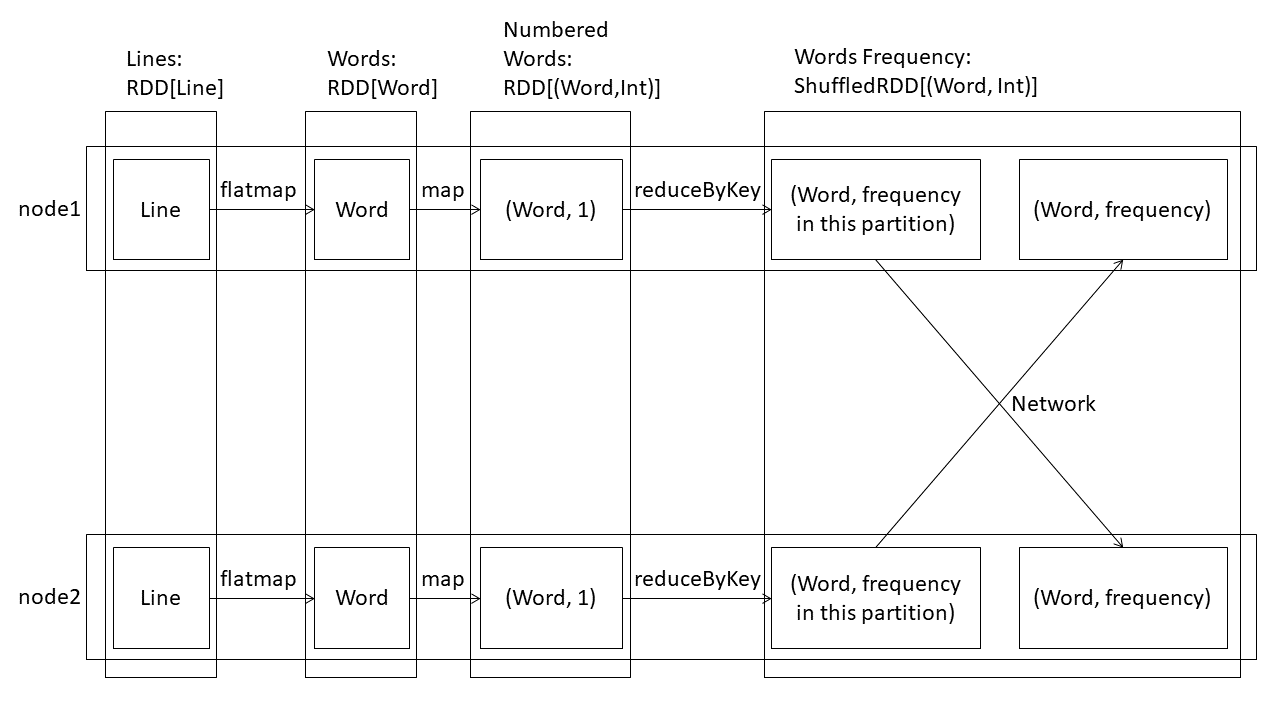
\includegraphics[scale=.4]{wordcount.png}}
    \end{center}
    \caption{ \label{figure:4} A Directed Acyclic Graph (DAG) representing the above code in a cluster of 2 nodes}
\end{figure}

RDDs are not just immutable but a deterministic (pure) function of their input. That means RDD can be recreated at any time.This helps in taking advantage of caching, sharing and replication. RDD isn't really a collection of data, but just a recipe for making data from other data. Immutability rules out a big set of potential problems due to updates from multiple threads at once. Immutable data is definitely safe to share across processes. Immutable data can as easily live in memory as on disk. This makes it reasonable to easily move operations that hit disk to instead use data in memory, and again, adding memory is much easier than adding I/O bandwidth. RDD significant design wins, at cost of having to copy data rather than mutate it in place. Generally, that's a decent tradeoff to make: gaining the fault tolerance and correctness with no developer effort worth spending disk memory and CPU on.

Also Note that (flatMap, map, reduceByKey) are all transformations and all of the above code wouldn't trigger any computation unless we call what Spark describe as an Actions.\newline
Actions include (collect, take, \dots). for example, calling .take(10) on lines would give us the first 10 lines and calling .collect() on wordsFrequencies would give us a (key,value) map (sometimes called dictionary, object, hashmap) that would reside in the Main Memory of the machine that ran the collect method.

Note that Shuffling is necessary in the case of reduceByKey since we are counting the words occurrences on the file level and thus we need to sum up occurrences of each word in each partition.

As we saw Spark power resides in it's core abstraction\dots RDDs which are immutable, lazy and deterministic, which makes them thread safe, distributed, And allows us to perform DAG based optimizations which reduce the amount of communication between nodes over the network which is a huge cause for latency.


\section{Conclusions}
We saw the advantages of leveraging immutability as a key architectural concept in designs of a number of new technologies and open source projects. And how contrary to popular believe that immutability introduces a performance overhead and wastes memory. implementation of immutability in multiple fields of state management prove otherwise and that immutability will eventually leads to better performance and broader horizons were we can achieve what was considered impossible in a matter of minutes (in the case of Spark).

% Another huge advantage lazy evaluation gives us is the ability to use DAGs to optimize complex and large jobs
% https://techvidvan.com/tutorials/apache-spark-dag-directed-acyclic-graph/


% https://www.citationmachine.net/bibliographies/aefbbb90-00f3-449b-b369-1148cb3d2bb0

\newpage
\pagenumbering{Roman}
\setcounter{page}{1}
\section{References}
[1] Berman, J. J. (2018). Immutability and Immortality. In Principles and practice of big data: Preparing, sharing, and analyzing complex information (pp. 80–85). essay, Academic Press. \newline
[2] Trcka, Nikola \& Aalst, Wil \& Sidorova, Natalia. (2009). Data-Flow Anti-patterns: Discovering Data-Flow Errors in Workflows. Proceedings of the International Conference on Advanced Information Systems Engineering (CAiSE). 5565. 425-439. 10.1007/978-3-642-02144-2_34. \newline
[3] Solarwinds: Top 4 Causes Of Storage I/O Bottlenecks \& How To Mitigate Them \newline
[4] Norvig, P. (n.d.). Teach yourself programming in ten years. Retrieved March 5, 2022, from \url{http://norvig.com/21-days.html#answers} \newline
[5] Axelsson, L. (2017). Immutability : An Empirical Study in Scala LUDVIG AXELSSON. \newline 
[6] Smith, Jonathan \& Jr, Gerald. (1988). Effects of Copy-on-Write Memory Management on the Response Time of UNIX Fork Operations.. Computing Systems. 1. 255-278.
[7] Kernighan, B. W., and Ritchie, D. M. The C Programming Lan-
guage, Second Edition. Prentice Hall, 1988. \newline
[8] Levrinc, R. (2008). LLFS : a copy-on-write file system for Linux [Diploma Thesis]. reposiTUm. \url{https://resolver.obvsg.at/urn:nbn:at:at-ubtuw:1-28018} \newline
[9] Narkhede, N., Shapira, G., \& Palino, T. (2017). Meet Kafka. In Kafka: Real-time data and stream processing at scale (pp. 3–5). essay, O'Reilly Media, Incorporated. \newline
[10] Apache Software Foundation. (n.d.). Introduction. Apache Kafka. Retrieved March 10, 2022, from https://kafka.apache.org/intro \newline
[11]  (n.d.). Retrieved March 11, 2022, from https://elm-lang.org/ 







\newpage
\section{Acknowledgements}
Thank you for your time

\printbibliography


\end{document}




%###############################################


%############# Must Use Resource ###############
%###############################################
% \subsection{Structural Sharing}
% \subsection{Cpp example}
% $https://www.youtube.com/watch?v=y_m0ce1rzRI\&t=4081s$
% \subsection{Copy-On-Write}
% \subsection{logfilesystem}
% \subsection{Append Logs}%not important
% effecient cow reduce the overhead of threading and parallel processing
% sth
% \subsection{MVC}
% \subsection{elm}
% sth
%TODO: https://elm-lang.org/news/blazing-fast-html
%TODO: talk about referential transparency
%TODO: use these links:
%TODO: http://typeocaml.com/2015/01/02/immutable/
%TODO: https://algs4.cs.princeton.edu/23quicksort/
%TODO: https://coderscat.com/quicksort-history-and-impls/
%TODO: https://www.codingninjas.com/blog/2020/09/26/mutating-non-mutating-algorithms-in-c/
%TODO: https://discourse.elm-lang.org/t/can-the-compiler-skip-virtual-dom/6300
%TODO: https://www.ncbi.nlm.nih.gov/pmc/articles/PMC3136027/
%TODO: https://en.wikipedia.org/wiki/Persistent_data_structure#Garbage_collection
%TODO: https://en.wikipedia.org/wiki/Funarg_problem
%TODO: https://blog.sigplan.org/2022/01/13/provably-space-efficient-parallel-functional-programming/
%TODO: https://en.wikipedia.org/wiki/Persistent_data_structure#Garbage_collection
%TODO: StateManegment
% prefered data structures
% dum data classes
% following strong type system
% funcional
% contexts static compiletime
% curring dynamic clojures
% compile optimizations
% lazyness
% transperncy substitiustion model
% GC or static refs
% chanllenging
% modularity
% time travelling debugger
% bref on 
% deterministic concurrency
% reactiveity
% modernday statless deployment
% 	docker or distributed or actor
% 	strong endpoint devices